
\documentclass[unicode, notheorems]{beamer}
%\usepackage{ dsfont }
\usepackage{ amsmath }
\usetheme[numbers, minimal,totalnumbers]{Statmod}
\newcommand{\Expect}{\mathbf{E}}
\usepackage[english,russian]{babel}
\usepackage{ amssymb }
\usepackage{ dsfont }



\usepackage[T2A]{fontenc}

\usepackage[utf8]{inputenc}
\usepackage[russian]{babel}
\usepackage{amsthm}
\usepackage[unicode, pdftex]{hyperref}


\newtheorem{theorem}{Теорема}[section]
\newtheorem{example}{Пример}[theorem]
\newtheorem{definition}{Определение}[theorem]
\newtheorem{target}{Цель работы}

\newcommand{\specialcell}[2][c]{%
  \begin{tabular}[#1]{@{}c@{}}#2\end{tabular}}

\title[Нейронные сети]{Нейронные сети. Общая структура (особый класс функций для оптимизации). Back propagation как вычислительный подход.}

\author[Волканова М., Третьякова А., Фёдоров Н.]{Волканова Маргарита, Третьякова Александра, Фёдоров Никита}
\institute[СПбГУ]{Санкт-Петербургский государственный университет \\
	Математико-механический факультет \\
	Кафедра статистического моделирования \\
	\vspace{0.4cm}

	
	\vspace{0.3cm}
}
\date{
	Санкт-Петербург\\
	2019г.
}

\subject{Beamer}

\begin{document}

\maketitle






 

\begin{frame}
	\frametitle{Постановка задачи аппроксимации особым классом функций}
	\begin{itemize}
\item $X$ --- множество объектов, $Y$ --- множество ответов;\\
\item $X^n = (x_i, y_i)_{i=1}^{n}$--- обучающая выборка, $x_i \in \mathbb{R}^p$;\\
\item $(x^1,\ldots,x^p)$ --- признаки объекта $x \in X$;
\end{itemize}
Рассмотрим стандартное построение предсказывающей модели:
\begin{equation*}
Q(a, X^n) = \frac{1}{n} \sum_{i=1}^{n} \mathscr{L}(a,x_i,y_i) \rightarrow \min_w,
\end{equation*}
\begin{equation*}
\text{где }a(x, w) = \sigma( \langle w,x \rangle ) = \sigma\left(\sum_{j=1}^{p} w_j x^j - w_0 \right),
\end{equation*}
$w_k \in \mathbb{R}$, $k=0,\ldots,p$; 
$\sigma: \mathbb{R} \rightarrow  \mathbb{R} $ --- функция активации;
$\mathscr{L}(a,x_i,y_i)$ --- функция потерь, $i=1,\ldots,n$.

\end{frame}


\begin{frame}
	\frametitle{Модель нейрона для задач машинного обучения}
	
	\textbf{Задача классификации}: $Y =\{ \pm 1 \}$, $a(x_j,w) = sign \langle w,x_j \rangle$,
	
	\[
	Q(w, X^{n})=\sum_{j=1}^{n} \mathscr{L} \left( a(x_j ,w), y_j \right) = \sum_{j=1}^{n} [y_j \langle w,x_j \rangle  < 0] \rightarrow \min_{w}.
	\]
	
	
	\textbf{Задача регрессии}: $Y= \mathbb{R}$, $a(x_j,w) = \sigma( \langle w,x_j \rangle )$,
	
	
	\[
	Q(w, X^{n})=\sum_{j=1}^{n} \mathscr{L} \left( a( x_j,w ), y_j \right)=\sum_{j=1}^{n}\left( \sigma( \langle w,x_j \rangle ) -y_j \right)^2 \rightarrow \min_{w}.
	\]
	
	При $\sigma(z) = z$ получаем многомерную линейную регрессию.\\
	

\end{frame}

\begin{frame}
	\frametitle{Модель нейрона МакКаллока–Питтса}
\begin{equation*}
a(x, w) = \sigma( \langle w,x \rangle ) = \sigma\left(\sum_{j=1}^{p} w_j x^j - w_0 \right),
\end{equation*}
\begin{itemize}
	\item $x^j \in \mathbb{R}^n$, $j=1,\ldots,p$, --- числовые признаки, входы;
	\item $w_j \in \mathbb{R}$, $j=1,\ldots,p$ --- весовые коэффициенты (синаптические веса); 
	\item $\sigma(z)$ --- функция активации;
	\item $w_0$ --- порог активации (смещение).
	
\end{itemize}

\begin{columns}
	\column{.4\textwidth}
	\begin{center}
			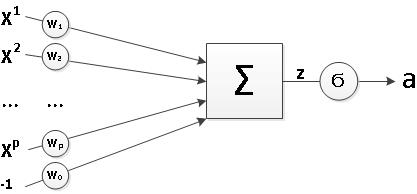
\includegraphics[width=1.15\linewidth]{dok}
		
	\end{center}
	\column{.4\textwidth}
	\begin{center}
		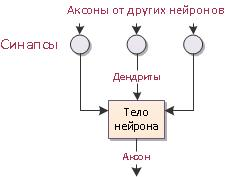
\includegraphics[width=1\linewidth]{bio_neurun}
	\end{center}
\end{columns} 
\end{frame}


	




\begin{frame}
		\frametitle{Булевы операции в виде нейронов}
		Унарная булева операция:
			$\neg x^1 = \left[-x^1 + \frac{1}{2} > 0 \right]$\\			
\begin{figure}
	\centering
	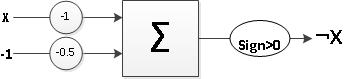
\includegraphics[width=0.5\linewidth]{no}
\end{figure}
		Бинарные булевы операции:
			
\begin{columns}
	\column{.5\textwidth}
	
	$x^1\vee x^2=\left[x^1 + x^2 - \frac{1}{2} > 0 \right]$
	\begin{center}
		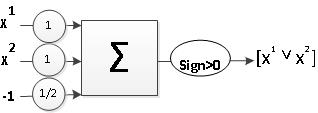
\includegraphics[width=0.9\linewidth]{or}\\
		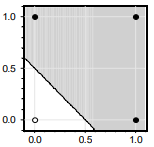
\includegraphics[width=0.4\linewidth]{screenshot002}
	
	\end{center}
	\column{.5\textwidth}
	$x^1 \wedge x^2 = \left[x^1 + x^2 - \frac{3}{2} > 0\right] $\\
	\begin{center}
		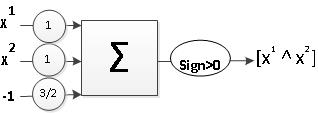
\includegraphics[width=0.9\linewidth]{and}\\
		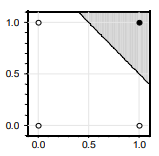
\includegraphics[width=0.4\linewidth]{screenshot001}
	\end{center}
\end{columns}

		
\end{frame}


\begin{frame}
	\frametitle{Функция XOR (Исключающее ИЛИ)}
	Функцию XOR не реализовать одним нейроном с двумя входами:
	\begin{enumerate}
		\item Добавление нелинейного признака:
		$	x^1 \oplus x^2 = \left[x^1 + x^2 - 2\textcolor{red}{x^1 x^2} - \frac{1}{2} > 0\right]$
		\begin{figure}
			\centering
			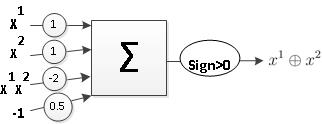
\includegraphics[width=0.5\linewidth]{xor11}
			\quad \quad \quad 
			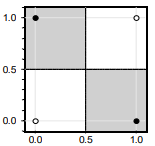
\includegraphics[width=0.2\linewidth]{screenshot003}
		\end{figure}
		
		\item \textcolor{red}{Сеть} (двухслойная суперпозиция) функций И, ИЛИ, НЕ:
		$x^1 \oplus x^2 = \left[ \neg \left( x^1 \wedge x^2 - x^1 \vee x^2 \right)  > 0\right].$
		\begin{figure}
			\centering
			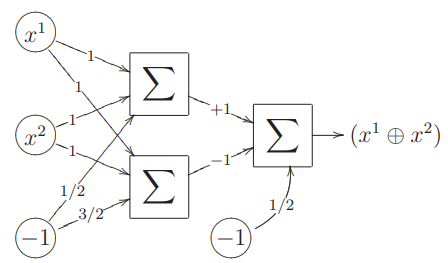
\includegraphics[width=0.35\linewidth]{screenshot006}
			\quad \quad \quad \quad \quad \quad \quad 
			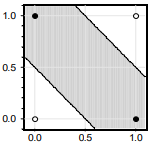
\includegraphics[width=0.2\linewidth]{screenshot004}
		\end{figure}
		\textbf{Нейронная сеть} --- суперпозиция нейронов.
	\end{enumerate}

\end{frame}

\begin{frame}
		\frametitle{Любую ли функцию можно представить нейросетью?}

\begin{theorem}[Цыбенко, 1989]
	Пусть $\sigma(x)$ --- непостоянная, ограниченная и монотонно возрастающая непрерывная функция; $C(I_{p_0})$ --- множество непрерывных функций на $[0,1]^{p_0}$.\\
	Тогда для любой $f \in C(I_{p_0})$ и $\varepsilon > 0$ существуют $p_1 \in \mathbb{Z}$ и  $\alpha_i$, $b_i$, $w_{ij} \in \mathbb{R}$, $i=1,\ldots,p_1$, $j=1,\ldots, p_0$, такие что для любого $x=(x^1, \ldots, x^{p_0}) \in I_{p_0}$ выполняется
\[	
	| F(x^1, \ldots, x^{p_0}) - f(x^1, \ldots, x^{p_0})| < \varepsilon,
\]
\[\text{где }
F(x^1, \ldots, x^{p_0})=\sum_{i=1}^{p_1} \alpha_i \, \sigma \left(\sum_{j=1}^{p_0} w_{ij} x^j + b_i.   \right)
\]
	
\end{theorem}
	\textcolor{red}{Вывод:} С помощью линейных операций и одной нелинейной функции активации можно приблизить любую непрерывную функцию с любой желаемой точностью. 
\end{frame}



\begin{frame}
	\frametitle{Функция активации и функция потерь}
	\textbf{Функции активации:}
	\begin{itemize}
		\item Сигмоида: $\sigma(z) = \frac{1}{1+e^{-a\,z}}$, $a \in \mathbb{R}$;

		\item Softmax: $SM_i(z)  = \frac{e^{z_i}}{\sum_{k=1}^{K}e^{z_k}}$;
		\item Гиперболический тангенс: $\sigma(z) = \frac{e^{a\,z} - e^{-a\,z}}{e^{a\,z} + e^{-a\,z}}$, $a \in \mathbb{R}$;
		\item Выпрямитель: $ReLU(p) = \max (0,p)$;
	\end{itemize}
	\textbf{Функции потерь:}($t$ - истинное значение, $p=\sigma(y)$)
		\begin{itemize}
		\item Среднеквадратичная ошибка: $MSE(p,t)=(p-t)^2$;	
		\item Бинарная кросс-энтропия: $BCE(p,t) = -t\log p - (1-t)\log (1-p)$;
		\item Кросс энтропия: $CE(p,t)=-\sum_{c=1}^{N}t_c \log p_c$;
	\end{itemize}
 
\end{frame}
\begin{frame}

	\frametitle{Многослойная нейронная сеть}
Пусть для общности $Y = \mathbb{R}^M$ и слоёв для простоты только два.\\
\vspace{0.4cm} 
\begin{columns}
	\column{.3\textwidth}
	$\quad$ входной слой, \\
	$\quad$ $p$ признаков\\
	$\quad$ $\overbrace{\quad \quad \quad \quad \quad}$
	\column{.3\textwidth}
	скрытый слой, \\
	$H$ нейронов\\
	$\overbrace{\quad \quad \quad \quad \quad}$
	
	\column{.3\textwidth}
	$\,\,\,$ выходной слой, \\
	$\,\,\,$ $M$ нейронов\\
	$\,\,\,$  $\overbrace{\quad \quad \quad \quad \quad}$
	
\end{columns} 

\begin{center}
	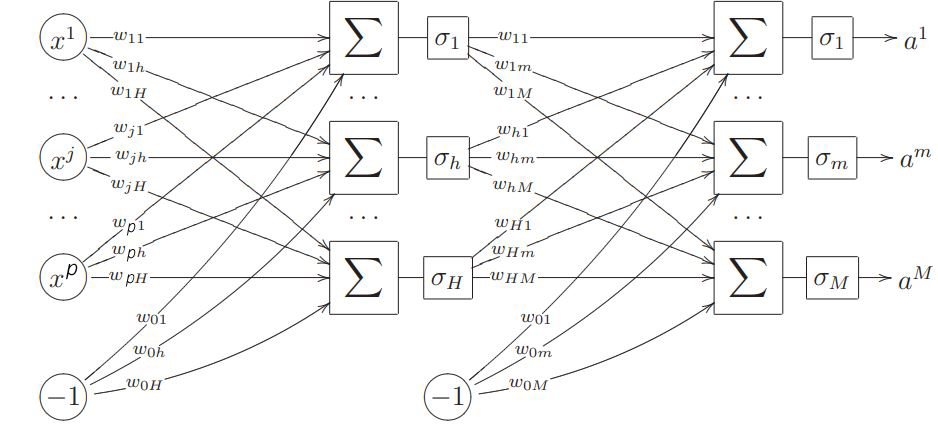
\includegraphics[scale=0.45]{all}
\end{center} 	


\end{frame}
\begin{frame}
	\frametitle{Напоминание: Стохастический градиентный спуск}
Идея: на каждом шаге учитывать только одно наблюдение. \\
	\[
Q(w)=\sum_{j=1}^{l} \mathscr{L} \left(  w,x_j, y_j \right) \rightarrow \min_{w}.
\]
\textcolor{blue}{\bfseries Вход:} $X^n = (x_i, y_i)_{i=1}^{n}$, $\lambda$, $\eta$;\\
\textcolor{blue}{\bfseries Выход:} синаптические веса $w \equiv (w_{jh}, w_{hm}) = (\{ w_{jh}\}_{j,h=0}^{p,H}, \{w_{hm}\}_{h,m=0}^{H,M}) \in \mathbb{R}^{H(p+M+1) + M}$;\\
\begin{enumerate}
	\item Инициализация веса $w$, выбор скорости обучения $\eta$, темп забывания $\lambda$, начальная оценка функционала 
$\overline{Q}(w)=\frac{1}{n} Q(w)=\frac{1}{n} \sum_{i=1}^n \mathscr{L}(w,x_i,y_i);$
\item \textcolor{blue}{\bfseries повторять}
\begin{enumerate}
	\item Случайный выбор $x_i$ из $X^n$ и вычисление функции потерь $\mathscr{L}_i:=\mathscr{L}(w,x_i,y_i)$;
	\item Градиентный шаг: $w:=w- \eta \textcolor{red}{\nabla \mathscr{L}(w,x_i,y_i)}$;
	\item Оценка функционала $Q :=(1-\lambda)Q+\lambda \mathscr{L}_i$;
\end{enumerate}	
\textcolor{blue}{\bfseries пока} значение $Q$ и/или $w$ не стабилизируется.
\end{enumerate}		
\end{frame}


\begin{frame}
	\frametitle{Дифференцирование суперпозиции функций}
	Выходные значения сети $a^m(x_i)$, $m=1,\ldots,M$ на объекте $x_i$:
	\[
	a^m(x_i) = \sigma_m \left(\sum_{h=0}^{H} w_{hm}  \textcolor{red}{ u^h(x_i)}  \right); \quad \quad \quad 
	\textcolor{red}{ u^h(x_i)} = \sigma_h \left(\sum_{j=0}^{p} w_{jh} x_{i}^j   \right).
	\]

	Пусть для конкретности $\mathscr{L}_i(w)$ --- средний квадрат ошибки:
	\[
	\mathscr{L}_i(w) = \frac{1}{2} \sum_{m=1}^{M}(a^m(x_i) - y^m_i)^2.
	\]
	
	\textbf{Промежуточная задача:} найти частые производные 
	\[
	\frac{\partial \mathscr{L}_i(w)}{\partial a^m}; \quad \frac{\partial \mathscr{L}_i(w)}{\partial u^h}.
	\]
\end{frame} 

\begin{frame}
	\frametitle{Быстрое вычисление градиента}
	\textbf{Промежуточная задача:} частая производная 
	\[
	\frac{\partial \mathscr{L}_i(w)}{\partial a^m} = a^m(x_i) - y_i^m = \varepsilon_i^m
	\]
	--- это ошибка на выходном слое.
	\[
	\frac{\partial \mathscr{L}_i(w)}{\partial u^h} = \sum_{m=1}^{M}(a^m(x_i) - y_i^m) \sigma^{'}_m w_{hm} =\sum_{m=1}^{M} \varepsilon_i^m  \sigma^{'}_m w_{hm} =\varepsilon_i^h
	\]
	--- назовём это \textit{ошибкой на скрытом слое}. \\
	\vspace{0.4cm}
	Похоже, что $\varepsilon_i^h$ вычисляется по $\varepsilon_i^m$, если запустить сеть <<задом наперёд>>:
	
	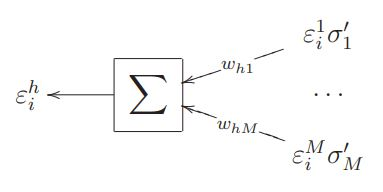
\includegraphics[scale=0.5]{fast}
	

\end{frame} 

\begin{frame}
	\frametitle{Быстрое вычисление градиента}
	Теперь, имея частные производные $\mathscr{L}_i(w)$ по $a^m$ и $u^h$, легко выписать градиент $\mathscr{L}_i(w)$ по весам $w$:
	\\
\small{
	\[\frac{\partial \mathscr{L}_i(w)}{\partial w_{hm}} = \frac{\partial \mathscr{L}_i(w)}{\partial a^m} \frac{\partial a^m}{\partial w_{hm}}=\varepsilon_i^m \sigma_m^{'} u^h(x_i), \quad h=0,\ldots,H, \quad  m=1,\ldots,M; \]
		\[
	\frac{\partial \mathscr{L}_i(w)}{\partial w_{jh}} = \frac{\partial \mathscr{L}_i(w)}{\partial u^h} \frac{\partial u^h}{\partial w_{jh}}=\varepsilon_i^h \sigma_h^{'} x_{i}^j, \quad j=0,\ldots,p, \quad h=1,\ldots,H.
	\]}
	\\
	\vspace{0.7cm} 
	%Под $ \sigma^{'}_m$ всегда будет подразумеваться производная в точке $\sum_{h=0}^{H} w_{hm} u^h(x_i)$. Аналогично, под $\sigma^{'}_h$ всегда будет подразумеваться производная в точке $\sum_{j=0}^{p} w_{jh} f_j(x_{i})$.  
\end{frame} 

\begin{frame}
	\frametitle{Алгоритм обратного распространения ошибки BackProp}
	\textcolor{blue}{\bfseries Вход:} $X^n = (x_i, y_i)_{i=1}^{n} \subset \mathbb{R}^p \times \mathbb{R}^M$; параметры $H$, $\lambda$, $\eta$.\\
	\textcolor{blue}{\bfseries Выход:} синаптические веса $w_{jh}$, $w_{hm}$. \\
	\begin{enumerate}
	\item инициализировать веса $w_{jh}$, $w_{hm}$;\\
	\item \textcolor{blue}{\bfseries повторять} \\
	    \begin{enumerate}
	\item случайно выбрать элемент  $x_i$ из выборки $X^n$; 
	\item прямой ход:\\
	$u_i^h := \sigma_h \left( \sum_{j=0}^{p} w_{jh} x^j_{i}\right), \,\, h=1,\ldots,H;$
	 $a_i^m := \sigma_m \left( \sum_{h=0}^{H} w_{hm} u_{i}^h \right), \,\, \varepsilon_i^m := a_i^m - y_{im}, \,\, m=1,\ldots,M;$
	$ \mathscr{L}_i := \sum_{m=1}^{M}(\varepsilon_i^m)^2, \text{ вычисление производных } \sigma_m^{'}, \sigma_h^{'}$;
	\item обратный ход:\\
	$\varepsilon_i^h := \sum_{m=1}^M \varepsilon_i^m \sigma^{'} w_{hm}$, $h=1,\ldots,H$;
	\item градиентный шаг:\\
	$w_{hm} := w_{hm} - \eta \varepsilon_i^m \sigma^{'}_m u_i^h$, $h=0,\ldots,H$, $ m=1,\ldots,M$;
	$w_{jh} := w_{jh} - \eta \varepsilon_i^h \sigma^{'}_h x^j_{i}$, $j=0,\ldots,p$, $ h=1,\ldots,H$;
	\item $Q := (1-\lambda) Q + \lambda\mathscr{L}_i$;
	
\end{enumerate}
	 \textcolor{blue}{\bfseries пока} $Q$ не стабилизируется.
	\end{enumerate}
\end{frame} 

\begin{frame}
	\frametitle{Преимущества и недостатки}
	\textbf{Преимущества:}
	\begin{itemize}
		\item эффективность: быстрое вычисление градиента;
		\item метод легко обобщается на любые $\sigma$, $\mathscr{L}$;
		\item возможно динамическое (потокое) обучение;
		\item на сверхбольших выборках не обязательно брать все $x_i$;
		\item возможность распараллеливания.
	\end{itemize}
	\vspace{0.7cm} 
	\textbf{Недостатки (есть все те же, что и у SG):}
	\begin{itemize}
		\item метод не всегда сходится;
		\item возможна медленная сходимость;
		\item застревание в локальных минимумах;
		\item проблема переобучения;
		\item сложно подбирать эвристики.
	\end{itemize}
\end{frame} 



  


\begin{frame}
	\frametitle{Улучшение сходимости и качества градиентного обучения}
		\begin{itemize}
	\item\textbf{Эвристики:} (те же, что и в обычном SG)
	\begin{itemize}
		\item инициализация весов;
		\item порядок предъявления объектов;
		\item оптимизация величины градиентного шага;
		\item регуляризация (сокращение весов). 
	\end{itemize} 
	\item\textbf{Более тщательный подбор начального приближения:}
	 Нейроны первого слоя настраиваются как $H$ отдельных однослойных сетей:
	\begin{itemize}
		\item либо по случайной подвыборке $X^{'} \subseteq X^n$;
		\item либо по случайному подмножеству входов;
		\item либо из различных случайных начальных приближений;
	\end{itemize}
	тем самым обеспечивается \textit{различность нейронов}.\\
\item Выбивание из локальных минимумов (jogging of weights).
 
	\end{itemize}
\end{frame} 

\begin{frame}
	\frametitle{Выбор градиентного метода}
	%	\begin{enumerate}
	%	\item  
	1. \textbf{Адаптивный градиентный шаг}. На каждом шаге ищем $\eta_*$:
	\[
	\mathscr{Q}(w - \eta \frac{\delta\mathscr{Q}}{\delta w}) \rightarrow \min_\eta.
	\]
	%	\item  

	2. \textbf{Диагональный метод Левенберга-Марквардта.}\\
	Метод Ньютона-Рафсона (второго порядка):
	\[
	w := w - \eta (\mathscr{Q}^{''}(w))^{-1} \mathscr{Q}^{'}(w),
\]
\small{	где $\mathscr{Q}^{''}(w) = \left( \frac{\partial^2 \mathscr{Q}(w) }{\partial w_{jh} \partial w_{j^{'}h^{'}}}   \right)$ --- гессиан размера $(H(p+M+1) + M)^2$}.\\

	\textbf{Эвристика.} Считаем, что гессиан диагонален:
\[
	w_{jh} := w_{jh} - \eta \left(  \frac{\partial^2 \mathscr{Q}(w) }{\partial w_{jh}^2} + \mu  \right) ^{-1} \frac{\partial \mathscr{Q}(w) }{\partial w_{jh}}, 
\]  
	$\eta$ --- темп обучения, \\
	$\mu$ --- параметр, предотвращающий обнуление элемента.
		%\end{enumerate}
\end{frame} 

\begin{frame}
	\frametitle{Оптимизация структуры сети}
	
	1. \textbf{Выбор числа слоёв.}
	
	Если знаем, что классы линейно разделимы, то можно ограничиться одним слоем. Двух-трёх слоёв обычно достаточно.  

		\vspace{0.6 cm}\\
	2. \textbf{Выбор числа нейронов в скрытом слое H.} \\ 
	\begin{enumerate}
		\item \textbf{Визуальный способ.} Если граница классов (или кривая регрессии) слишком сглажена --- количество нейронов в слое нужно увеличить, а если есть резкие колебания, то, наоборот, уменьшить (для задач с небольшим числом признаков).
		\item \textbf{По внешнему критерию.} 
		\begin{itemize}
			\item Средняя ошибка на тестовой выборке; 
			\item Cross-validation;
		\end{itemize}
		 Недостаток этого способа --- высокая трудоёмкость.
	\end{enumerate}
	
\end{frame}


\begin{frame}
	\frametitle{Динамическое наращивание сети}
	
	
	\begin{enumerate}
		\item Обучение сети при заведомо недостаточном числе нейронов $H \ll n$, пока ошибка не перестаёт убывать;
		\item Добавление нового нейрона и его инициализация путем обучения 
		\begin{itemize}
			\item либо по случайной подвыборке $X^{'} \subseteq X^n$;
			\item либо по объектам с наибольшими значениями потерь;
			\item либо по случайному подмножеству входов;
			\item либо из различных случайных начальных приближений.
		\end{itemize}
		\item Снова итерации BackProp;
	\end{enumerate}

\\

\textcolor{blue}{\bfseries Эмпирический опыт:} 
				\begin{itemize}
		\item\small{После добавления новых нейронов ошибка, обычно, сначала резко возрастает, затем быстро сходится к меньшему значению.}
			\item	\small{
		Общее время обучения обычно лишь в $1.5$--$2$ раза больше, чем если бы в сети сразу было нужное количество нейронов. Полезная информация, накопленная сетью, не теряется при добавлении новых нейронов.} 
	\item 	 \small{Полезно наблюдать за внешним критерием: прохождение $Q(X^k)$ через минимум является надежным критерием останова.} 
			\end{itemize}

\end{frame} 

\begin{frame}
	\frametitle{Удаление избыточных связей (OBD --- Optimal Brain Damage)}
	Пусть $w$ --- локальный минимум $Q(w)$,\\ тогда $Q(w)$ можно аппроксимировать квадратичной формой:
	\begin{equation*}
	Q(w + \delta) = Q(w) + \frac{1}{2} \delta^{\mathrm{T}} Q^{''}(w) \delta + o(\| \delta\|^2),
	\end{equation*}
	\small{где $Q^{''}(w) =  \frac{\partial^2 Q(w) }{\partial w_{jh} \partial w_{j^{'}h^{'}}}$ --- гессиан размера $(H(p+M+1) + M)^2$.}\\

	\textbf{Эвристика.} Пусть гессиан $Q^{''}(w)$ диагонален, тогда
	\begin{equation*}
	\delta^{\mathrm{T}} Q^{''}(w) \delta = \sum_{j=0}^{p}\sum_{h=0}^{H} \delta^2_{jh}   \frac{\partial^2 Q(w) }{\partial w_{jh}^2 }  +  \sum_{h=0}^{H}\sum_{m=0}^{M} \delta^2_{hm}   \frac{\partial^2 Q(w) }{\partial w_{hm}^2 }.
	\end{equation*}
	Хотим обнулить вес: $w_{jh} + \delta_{jh}=0$. Как изменится $Q(w)$?\\

	\begin{definition}
	\textit{Значимость (salience)} веса $w_{jh}$ --- это изменение функционала $Q(w)$ при его обнулении: $S_{jh} = w^2_{jh}  \frac{\partial^2 Q(w) }{\partial w_{jh}^2 } $.
	\end{definition} 
\end{frame} 

\begin{frame}
	\frametitle{Удаление избыточных связей (OBD --- Optimal Brain Damage)}
	\begin{enumerate}
		\item В BackProp вычислять вторые производные $\frac{\partial^2 Q(w) }{\partial w_{jh}^2 } $,  $\frac{\partial^2 Q(w) }{\partial w_{hm}^2 } $.
		\item Если процесс минимизации $Q(w)$ пришел в минимум, то
		\begin{itemize}
			\item упорядочить веса по убыванию $S_{jh}$;
			\item удалить $d$ связей с наименьшей значимостью;
			\item снова запустить BackProp.
		\end{itemize}
		\item Если $Q(w, X^n)$ или $Q(w, X^k)$ существенно ухудшился, то вернуть последние удаленные связи и выйти.
	\end{enumerate}
	\vspace{0.4cm}
	Аналогично, OBD можно использовать для 
	отбора информативных признаков для нейрона скрытого слоя.\\
	Суммарная значимость признака: $S_j = \sum_{h=1}^{H} S_{jh}$.\\
	\vspace{0.4cm}
	\textbf{Эмпирический опыт:} сеть, построенная с помощью OBD, 
 меньше склонна к переобучению, чем сеть сразу построенная по полученной структуре (со случайно инициализированными весами).
\end{frame} 


% \bibliographystyle{gost2008ns}

\end{document}